In this section, we present the evaluation of our NAT system, considering both software (SW NAT) and hardware (HW NAT) implementations. Two ablation settings (HW NAT without translation, without NAT) are introduced to measure the overhead of our HW NAT design. We conduct two evaluations:

\begin{itemize}
    \item We measure the throughput with different packet sizes ranging from 0 to 5000 bytes.
    \item We measure the throughput with different numbers of connections from 0 to 1024.
\end{itemize}

\subsection{Evaluation Setting}

We provide details for our settings in the two evaluations. The connection hash table size is configured as 1024 for both evaluations. A C language-based traffic generator continuously sends TCP packets to the desktop machine via a Linux packet socket to the 10GbE interface of the board in an infinite loop. The throughput is measured by dividing the data amount over the time of sending it. The data amount is set to 100 gigabits.

The four settings are:

\begin{itemize}
    \item \textbf{HW NAT}: Our hardware-based NAT system as described in the System Design and Implementation sections. It uses a bidirectional hash table to store mappings of LAN 5-tuple and WAN 5-tuple, XOR as the hash function, and linear probing as the collision resolution strategy. It achieves high-speed data conversion and forwarding, improving throughput.
    \item \textbf{SW NAT}: A software-based NAT system running on four threads, using a shared hash table with linear probing. The table size is 1024, serving as a baseline compared to HW NAT.
    \item \textbf{HW NAT w/o translate}: Similar to HW NAT, but using packets that do not require translation (e.g., ICMP packets) to measure performance.
    \item \textbf{w/o NAT}: No NAT at all, with packets directly forwarded between MAC/GTH and DMA. This is the ideal scenario and serves as an upper bound to evaluate the performance of our system.
\end{itemize}

\textbf{Latency:} We do not measure latency since the overhead of HW NAT is predictable, averaging only constant cycles when the load factor is much lower than the table size. Even in extreme situations where the load factor is 1, the maximum latency is only $tableSize \times cycleTime$, which is less than 10 $\mu s$ when the table size is 1024. It accounts for about 10\% of the normal ping-pong latency (100-200 $\mu s$) measured with the \verb|ping| command.

\subsection{Results}

\begin{figure}[t]
    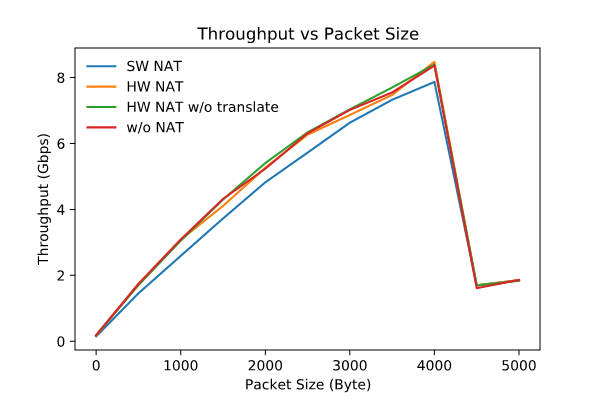
\includegraphics[width=\linewidth]{images/Result1.png}
    \caption{Throughput vs. Packet Size}
    \label{fig:thputpktsize}
\end{figure}

Figure \ref{fig:thputpktsize} depicts the relationship between throughput and packet size. As the packet size increases, the throughput also increases until it reaches a maximum value at around 4000 bytes, then suddenly drops. This phenomenon is observed in all four settings.

\begin{figure}[t]
    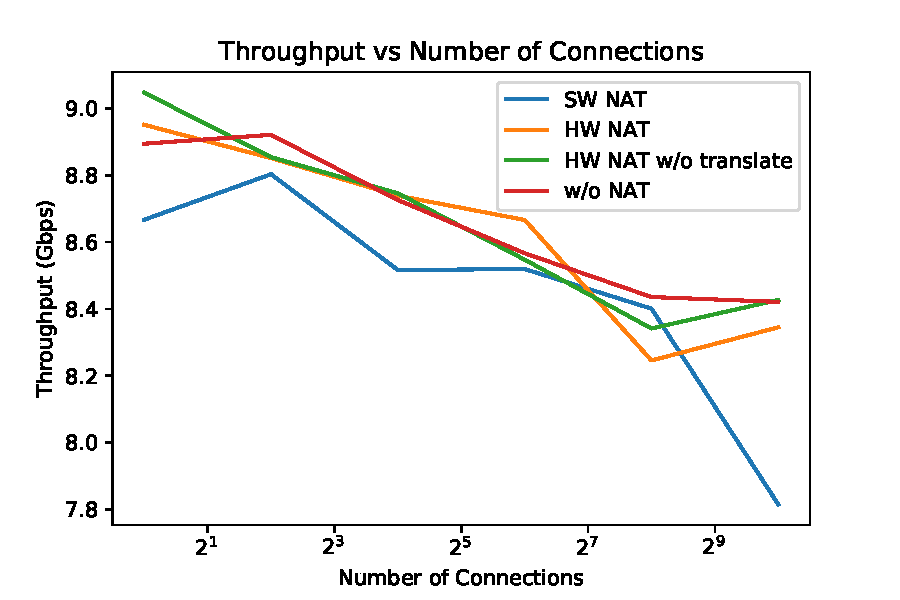
\includegraphics[width=\linewidth]{images/connection_throughput_log.pdf}
    \caption{Throughput vs. Number of Connections}
    \label{fig:thputconn}
\end{figure}

Figure \ref{fig:thputconn} illustrates the relationship between throughput and the number of connections. As the number of connections increases, the throughput of SW NAT drops sharply, while the throughput of other scenarios remains stable.

\subsection{Interpretation}

Our results lead to three main conclusions:

\begin{itemize}
    \item \textbf{The performance of HW NAT is up to 7.7\% higher than SW NAT under our setting.} In Figure \ref{fig:thputpktsize}, HW NAT and SW NAT reach maximum throughput under the same packet size. The maximum throughput of HW NAT is 8.48 Gbps, while the maximum throughput of SW NAT is 7.87 Gbps. This demonstrates that the HW NAT system can benefit from CPU savings.
    
    \item \textbf{Figure \ref{fig:thputpktsize} shows that SW NAT is a bottleneck, and HW NAT is not.} The performance gap between SW NAT and no NAT indicates that SW NAT is a bottleneck that degrades the overall system performance. Conversely, HW NAT shows performance improvement compared to SW NAT, suggesting that hardware implementation outperforms software. There is almost no performance gap between HW NAT and no NAT, indicating that hardware implementation has little impact on the original system performance.
    
    \item \textbf{Figure \ref{fig:thputconn} shows that SW NAT is unscalable, and HW NAT is scalable.} SW NAT does not scale well with the number of connections due to the CPU overhead of software NAT and the synchronization overhead of sharing the NAT table. In contrast, HW NAT scales well with the number of connections, using a bidirectional hash table and an arbiter design to handle NAT mappings.
\end{itemize}

\subsection{Anomalies}

There are two anomalies in our evaluation results. We offer speculative explanations for them.

\textbf{Why does the packet size need to be large to achieve line rate?} We speculate that this is due to the poor performance of the ARM cores and the not-so-efficient performance of DMA, MAC, and GTH IP. The FPGA side has to process the packets at high speed, and may not handle small packets efficiently. Therefore, the packet size needs to be large enough to saturate the bandwidth of the FPGA side.

\textbf{Why is there a cliff-like drop after 4000 bytes?} We speculate that this is due to the existence of a 4K buffer in the link, causing extra overflow handling for large packets. When the packet size exceeds 4K, the buffer may not store the entire packet, leading to packet segmentation and additional overhead, which reduces throughput.
